\documentclass{article}
\usepackage[english]{babel}
\usepackage[utf8]{inputenc}
\usepackage{amssymb}
\usepackage[super]{natbib}
\usepackage{natbib}
\usepackage{graphicx}
\usepackage{blindtext}
\usepackage{listings}
\usepackage{amsmath}
\usepackage[utf8]{inputenc}
\usepackage{hyperref}
\usepackage{listings}
\usepackage[svgnames]{xcolor}
\lstset{language=R,
    basicstyle=\small\ttfamily,
    stringstyle=\color{DarkGreen},
    otherkeywords={0,1,2,3,4,5,6,7,8,9},
    morekeywords={TRUE,FALSE},
    deletekeywords={data,frame,length,as,character},
    keywordstyle=\color{blue},
    commentstyle=\color{DarkGreen},
}

\title{\textbf{The Stochastic Gradient Descent and a implementation/simulation in R}}

\date{April 2021}
\author{Anonym\\ \textit{University of Vienna}}
\begin{document}

\maketitle

\begin{abstract}
This paper will give you a basic introduction into the stochastic gradient descent, shows the difference in relation to the gradient descent and will set out some of the most important issues and solutions of an implementation by a simulation in context of a linear model. 
\end{abstract}


\section{Introduction}
Efficiency in terms of solving problems fast and sufficient is one of the most wanted properties regarding to algorithms fighting with big data these days. To generate information out of data you need to define your data as a mathematical optimization problem and choose a method that you believe is solving the problem properly. Common and simple models can work with exact numeric solutions, for example, the Ordinary Least Squares (OLS) method for linear regressions. In some cases, you can call some of the estimators using these methods efficient. Mathematically, that means, that the variance of this estimator is minimal in a certain class of estimators. But when it comes to huge data sets, you would not call the OLS method efficient, since we still have limits of computing capacity. This paper is about one of the most ancient and most efficient optimization methods, when it comes to big data and neuronal networks: The stochastic gradient descent (SGD). Since Herbert Robbins and Sutton Monro \cite{Herbert} published their paper on "A Stochastic Approximation Method" in 1951, the SGD became very popular. It just seems to work surprisingly well for a wide range of statistical models in machine learning. Although there are still open research problems like showing and proving certain properties of common applied sub-methods of the SGD. The convergent behavior, for example, is extremely sensitive to the methods parameters one has to set and it is still a problem to define its best parameters. This article will give you an introduction from an applied point of view into the SGD first, and will end up with an implementation and a simulation of the SGD on context of a linear model.  
\pagebreak

\section{Stochastic Gradient Descent}
\subsection{Introduction}
The goal of the Gradient Descent and of the SGD as well is to find a minimum of a function. Both methods iterate towards the opposite direction of the gradient, which will lead to a minimum under certain conditions. In case of an application the function is called a loss or cost function, which can be defined as follows: 
\begin{equation}
\label{eq:1}
\min_{x\in{X}}\frac{1}{n}\sum^{n}_{i=1}{f_i(x)} 
\end{equation}
We do not constrain \textit{x} and focus on finite sums, since we want to apply this method for real data sets, which have finite data points \textit{n} where $ X \in \mathbb{R}^d $ , so the dimension of each data point is $ d \in \mathbb{N}$.  Both parameters can be very huge. When we think of data points as images, \textit{d} would be around a million and of course \textit{n} can be very large too. In case of big companies like Facebook, Google and co., one dimension could be the amount of users, which would be around some billions. Additionally we have to assume that the function $ {f_i(x)} $ is at least once differentiable for all $i \in \{1,...,n\} $. 

The sum defines the actual difference between both methods, whereby the gradient descent is summing up over all data points which is done in (\ref{eq:1}), whereas the SGD is summing up over one or just a small group of random chosen data points. It is a very small change in the notation and definition, but actually leads to a big difference in properties. Considering that both methods are approximating roots of the loss function with an iterative process, we are interested in the most important conditions for the convergent behavior of this process. Indeed, the behavior is constrained by the loss function. Kiwiel and Krzysztof C.\cite{Kiwiel} proofed that the gradient descent converges linear under appropriate conditions. The strongest property which comply these conditions is convexity. If the function is convex, we do not have to worry too much about the iterative process getting stuck at a certain point or just converging too slow. So we keep that in our mind, when we will take a look at different loss functions later on. The SGD´s convergent behavior is instead really not that easy to sum up, but also for convex functions Léon Bottou and Frank E. Curtis and Jorge Nocedal \cite{bottou} showed that the SGD converges fast linear for the first iterations and then converges to some neighborhood of the solution of the loss function. In case of machine learning this is satisfying enough, because perfect solutions often end in over-fitting the model.
\pagebreak

\subsection{Loss functions}
To get a better understanding of the loss function, we can take a look on a few different examples.  We also define an index set \textit{I}. For instance the gradient descent takes all data points into the sum, so \textit{i} \begin{math}\in \{1,...,n\}\end{math}  and for the SGD we would just pick one random integer for each iteration. Other sub-methods of the SGD would use a small groups or so called batches of random or partly random chosen integers.
Let's take a look at least-squares loss function first, in which we write \textit{x} in terms of \(\hat{\beta}\): 
\begin{equation}\label{eq:2}
f_i(\hat{\beta}) = \sum_{i \in I}(y_j - X_{.,i}\hat{\beta})^2
\end{equation}
Here is \( \hat{\beta} \in \mathbb{R}^d \) and \( X_{.,i} \) is the \(i^{th} \) row of a data set \( X \in \mathbb{R}^{n\times d} \). This quadratic function is always convex regardless of the input of \textit{X},  hence we can easily apply the SGD or other methods to find the minimizer.

The Lasso loss function:
\begin{equation} 
f_i(\hat{\beta}) = \sum_{i \in I}(y_j - X_{.,i}\hat{\beta})^2 + \lambda \sum_{k=1}^d|\hat{\beta_k}|
\end{equation}
This function gets a little bit more complex by adding up a penalty term in form of the absolute values of \(\hat{\beta}\). It is no longer quadratic, but still convex.

Support vector machines: 
\begin{equation} 
f_i(w,b) = \lambda||w||^2+\frac{1}{\#I}\sum_{i \in I} \max(0,1-y_i(w^Tx_i-b))
\end{equation}
Here denotes \# the quantity of a set. Solutions for this loss functions are one of the most robust prediction methods to classify data points. In general you can formulate a lot of applied problems to this form, like the classification of images. More accurate the classification of proteins \cite{Gaonkar}, satellite data \cite{maity2016supervised} or even handwritten characters \cite{7333916} \cite{Dennis}. 
This function is also convex.

Maximum-Liklihood:
\begin{equation} 
f_i(\theta) = - \frac{1}{\#I} \sum_{i \in I} l(\theta)
\end{equation}
In general the Maximum-Liklihood function is not concave, so the negative not convex, and depends on its parameters. Just in case of a simple regression model including an ordinal dependent variable, it has been proofed that the LogLiklihood function is concave if the derivate of the underlying response function has concave logarithm. For more information about the properties of different Lilkihood functions the reader can take a look at "Concavity of the Log Likelihood" of John W. Pratt (1981)\cite{doi:10.1080/01621459.1981.10477613}. We see that the loss function has a lot of different forms, but often can be formulated, at least in this examples, in form of a convex function, which is very useful when we want to apply the SGD.

\subsection{SGD Iteration}
We know that the derivative of a function can be used to find an extremum. More precisely, the zero derivative of a function might indicate a minimum, maximum or a saddle point, in case the function is not convex. The goal of the SGD is to find this zero derivatives by an iteration, which should decrease the gradient by every step, until it is approximately zero or in an satisfying neighborhood of the solution. Because the Gradient is giving the fastest increase at a certain point, this iteration takes the negative value to find the fastest decrease:
\begin{equation}
x_{k+1} = x_k - \eta_k \Delta f_i(x_k)
\end{equation}
Here \( \Delta f_i(x_k)\) denotes the Gradient, which is defined as the vector containing all partial derivatives of the loss function with respect to each component:
\begin{equation} 
 \Delta f_i(x_k) = ( \frac{\delta f_i(x_k)}{\delta {x_k}_1}, \frac{\delta f_i(x_k)}{\delta {x_k}_2}, ... , \frac{\delta f_i(x_k)}{\delta {x_k}_d}) 
\end{equation}
Beyond that the starting point \(  x_0 \) has to be chosen first and should be, if possible, in the near of the solution. Furthermore we have to define \( \eta_k \), which is called the learning rate or step size. It determines the impact of \( \Delta \) on the new update \( x_{k+1}\). There are a lot of different methods to define the step size. As mentioned at the beginning, it is still a problem to find the best step size for the algorithm, but there are a lot of adaptive methods to find at least a "good" step size, which mainly ensure that the SGD will converge. Herbert Robbins and Sutton Monro (1951)  \cite{Herbert} found the conditions for \( \eta_k \), which almost surely guarantee the convergence of a global minimum within a convex function: 
\begin{equation} 
\sum_{k = 1}^{\infty}\eta_k = \infty \; \; \; \textrm{ and } \; \; \; \sum_{k = 1}^{\infty}\eta_k^2 < \infty
\end{equation}
One example of \( \eta_k \) full filing these conditions is to define \( {(\eta_k)}_{k=1}^\infty \) such, that we obtain the harmonic series:
\begin{equation}\label{eq:9}
\eta_k = c(\frac{1}{k}) \; \;\textrm{ , }\; \; c \in \mathbb{R}
\end{equation}

The first condition is complied, because we have a harmonic series, and the second condition is known as the Basler problem and is also full filled: \begin{equation}
\sum_{k = 1}^{\infty}\frac{c}{k^2} = \frac{c\pi^2}{6} < \infty 
\end{equation}

However,  more recent  formulations for \( \eta \)  use adaptive step sizes,  which are expressed in a function  of past stochastic gradient terms. In addition, most of those functions include more variables, which one has to set and on which one has to think about before applying the SGD. The most common adaptive step size will look like this: 
\begin{equation}\label{eq:11}
\eta_k = \frac{\alpha}{(\beta + \sum_{i=1}^{k-1}||f_i(x)||^2)^{\frac{1}{2+\epsilon}}}
\end{equation}
Where \( \alpha > 0\) and \( \beta, \epsilon \geq 0\). Duchi et al. (2011) came up with this generalize form in "Adaptive subgradient methods for online learning and stochastic optimization"\cite{duchi2011adaptive}, where they set out a lot of improvements of the step size regarding to distribution of the data and in general they found out that adaptive methods clearly outperform their non adaptive methods. So if the SGD takes too much time to perform or does not converges for a given amount of iterations, it is very useful to adjust the step size intending to improve the algorithm. 

\section{Simulation and Implementation in R}
This abstract is about to give a better understanding of the most important parameters of the SGD, when it comes to an implementation in R. The focus is set on the questions: 
\begin{itemize}
    
    \item What impact has the \textit{number of iterations} on the behavior of the SGD? 
    \item What impact has the \textit{learning rate} or \textit{step size} on the behavior of the SGD? 
    \item What impact has the \textit{starting point} $X_0$ on the behavior of the SGD? 
    \item When is the SGD faster than the computation of the OLS-Estimator in context of a linear model?
\end{itemize}
It is obvious, that the SGD behavior is different in case of different models and data sets. It is not possible to give an answer to all those questions and scenarios in a mathematical correct and well-defined way, and that is why it is important to define an environment, in which the simulation takes place and in which the results can be interpreted. The results will help to get the right feeling of what potentially can happen and what potentially will work out when applying the SGD in a similar environment.
\subsection{Environment}
We will focus on a common linear model:
$$ Y = X\beta + \epsilon  \quad \text{ with } \quad \epsilon_i \sim \mathcal{N}(0,1) $$
The standard assumptions are complied and there is no need to go through  them in detail, since we will generate the data. For this model we want to find the solution for beta which minimize the loss function (\ref{eq:2}) shown at page three. This function is a convex function, for which we already know, that the SGD should converge fast linear by the first iterations and then should end up in a neighborhood of the solution. In the following we will see what exactly this means.
\pagebreak 
Furthermore, we will generate the data such that we can assume that the solution of the loss function is: $$\hat{\beta} = (1,1) $$ The solution two-dimensional, because there is a nice way of plotting the iterations in a two-dimensional space. Of course, the SGD works for any number of dimensions as well.

\subsection{What impact has the \textit{number of iterations} on the behavior of the SGD?}
Let’s study the impact of different number of iterations. We start with 5, 10, 20, 50, 500 and 2000 iterations. We will use an adaptive step size in form of the harmonic series (\ref{eq:9}) for $ \eta_k $ , whereby $ c = 1 $. Furthermore, we set the starting point to (15,15), which is  marked green. The last iteration is marked purple and the solution (1,1) red, whereby a circle is drawn around the solution with radius of 4, which can be interpret as neighborhood. Also they help to recognize the possibly different scaling for each plot. We will obtain a different plot for each performance, because the data point $ x_i $ is chosen randomly for each iteration and each run of certain iterations.

\begin{figure}[h]
    \centering
    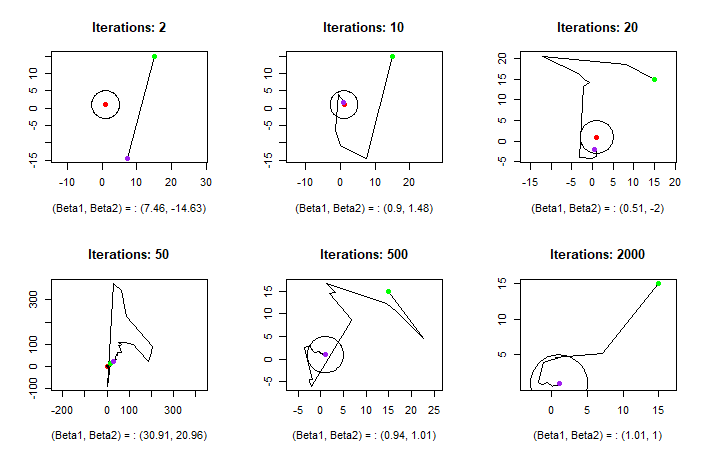
\includegraphics[width=\textwidth]{Iterations 2.png}
    \label{fig:mesh1}
\end{figure}

If one look at the plots, something is very eye-catching: One can observe some random fluctuation in the way the SGD approximate the solution. This random fluctuation is based on the random choice of the one data point. This data point $x_i$ can lay on the regression line, for which the gradient would be the same as if the whole data set would be included. But the data point mostly lays above or underneath the regression line, which is why the SGD can sometimes run in a direction not going to the solution straight. For this reason the SGD is sometimes not improving with a new iteration. This can be seen in an early iteration like in the 5th plot (Iteration: 500), where the 2nd iteration seems not to improve the first iteration. Also for late iterations this is not uncommon, but is hardly to see in the plots, since the step size gets smaller and smaller with each iteration. The second kind of an abnormality is the 4th plot, which looks very strange. The solution got even worse than the starting point. This is not the general case and is rarely seen, when repeating the simulation again. The chosen adaptive step size (\ref{eq:9}) or very bad first data points could be the reason for this failure. Because the step size has a big impact on the change, it is hard to get to the solution again fast, after the first iterations led into the wrong direction or after the first iterations overshot the solution. 

Despite this outcome the SGD should actual improve in expectation with every new iteration, which is shown the following simulation, where the SGD was repeated 1000 times for each iteration and the distance to the solution was plotted in a histogram.

\begin{figure}[h]
    \centering
    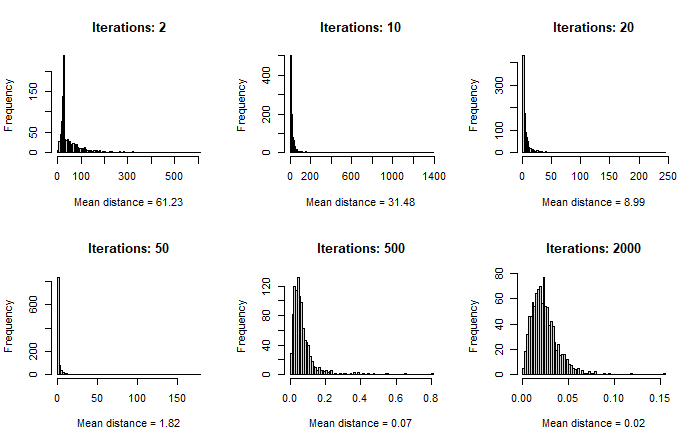
\includegraphics[width=\textwidth]{Simulation(diffIterations)2.png}
    \label{fig:mesh2}
\end{figure}

That the distance would get smaller was to be expected. However, this result shows again, what is meant by fast linear convergence by the first iterations. In particular we observe a better improvement in proportion to the increase by the first 500 iterations. The last improvement from 500 to 2000 then does not seem to be that fast. 

\pagebreak
A last visualization shows the distribution of ending points with different iterations. The higher the number of iterations the brighter the color of the points:
\begin{center}
    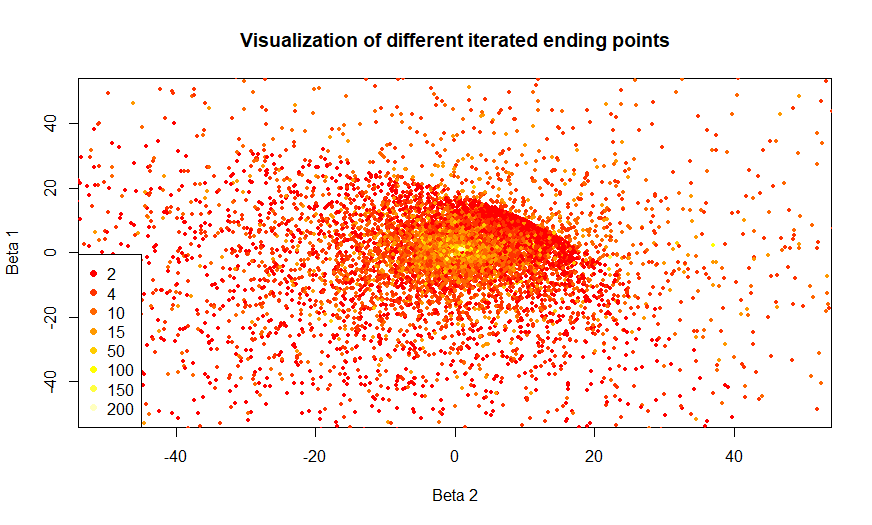
\includegraphics[width=\textwidth]{Visulization Dots.png}
\end{center}
 As expected, the density of brighter points is higher in the area of the solution (1,1), which is not that surprising, since this was a result of the simulation done before. Anyway, it is interesting that there is a structure in form of a red line, which has something to do with the starting point. Since the starting point is fixed at (15,15), the direction for the first iteration is more or less also fixed within 180 degrees, which leads to this structure. 

\subsection{What impact has the \textit{learning rate} or \textit{step size} on the behavior of the SGD? }
In the previous chapter an adaptive step size was already used for a good reason. Clearly, there are different forms of adaptive step sizes, but anyway they should always be preferred to non adaptive step sizes regarding to Duchi et al. (2011). \cite{duchi2011adaptive} To get this clear, we first take a look at non adaptive step sizes, plot the distributions of 1000 simulations as before and then do the same simulation for the adaptive etas. The number of iterations was set to 200: $$\textrm{Non-adaptive: } \eta_k = c \quad \quad \textrm{with } c \in \{  1,\: 0.5,\: 0.25,\: 0.1,\: 0.05,\: 0.0000005 \} $$ 
$$\textrm{Adaptive: } \eta_k = \frac{4}{k} , \quad \eta_k = \frac{2}{k} ,\quad  \eta_k = \frac{1}{k} ,\quad  \eta_k = \frac{1}{2k} ,\quad  \eta_k = \frac{1}{3k} ,\quad  \eta_k = \frac{1}{4k} $$

\begin{center}
    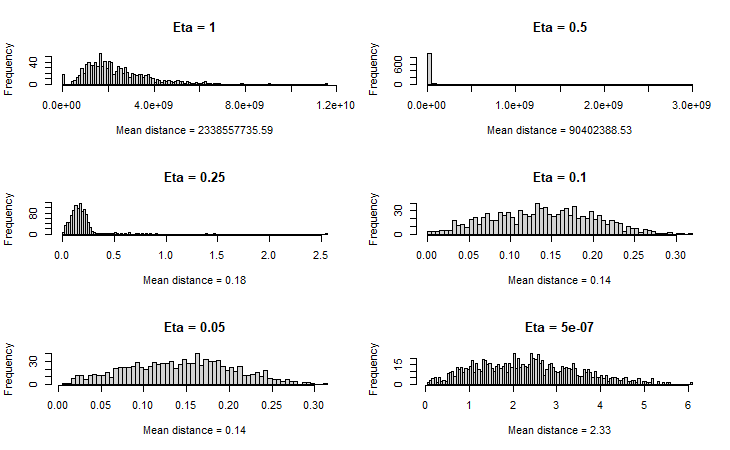
\includegraphics[scale=0.57]{Constant Etas.png}
\end{center}


This figure shows the sensibility of the SGD regarding to the step size. One can see that the first eta diverged for nearly every execution (The last calculable value is taken to make the result presentable). Also the second eta diverged for most of the runs. For a smaller eta the methods seems to work better, but of course there is also a lower bound for which the algorithm gets worse again, which is in this example between the last two etas. In general one should rather choose eta a little bit too small than too high. The method will hardly diverge for an eta near 0. In fact, the chance of the algorithm diverging for an arbitrarily small eta moves towards zero, at least for convex functions. In return the convergence slows down as seen for the last eta. The following figure shows the distribution for the adaptive step sizes: 

\begin{center}
    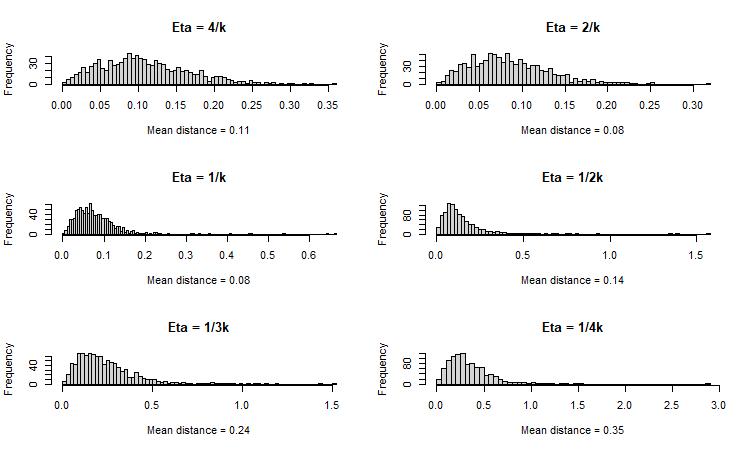
\includegraphics[scale=0.57]{Eta adaptive.png}
\end{center}

These results suggests that adaptive methods are way more robust. Moreover, one can see an improvement of best non adaptive method (eta = 0.05) with a mean distance of 0.14 to the best adaptive method (eta = 1/k) with a mean distance of 0.08. This is significantly closer to the solution relatively spoken. Furthermore, the adaptive methods converge faster, which can be found out by testing different number of iterations, but was not a focus of this examination. The last adaptive method (\ref{eq:11}) was also tested for a set of alphas and betas, but in fact there was not an obvious improvement to the first adaptive methods. Still, it was even more robust than the first adaptive methods, which means that the parameters are more independent to the convergent behavior. The highest mean distance for the chosen set of alphas and betas was approximately 16, which can be seen in the following table for alpha = 100 and beta = 0.1.
\begin{table}[ht]
\centering
\begin{tabular}{rrrrrr}
  \hline
$ \alpha \diagdown $ \beta & 100 & 10 & 1 & 0.1 & 0.01 \\ 
  \hline
100 & 1.26 & 0.72 & 4.54 & 16.05 & 4.59 \\ 
  10 & 0.57 & 0.56 & 0.58 & 0.56 & 0.87 \\ 
  1 & 0.18 & 0.23 & 0.21 & 0.23 & 0.21 \\ 
  0.1 & 0.34 & 0.18 & 0.15 & 0.14 & 0.13 \\ 
  0.01 & 1.68 & 1.61 & 1.59 & 1.59 & 1.58 \\ 
   \hline
\end{tabular}
\end{table}


As mentioned, the best alpha and beta is not that easy to find and one can do a lot of preparatory work and calculations to do so. Fore more information the reader is referred to "Adaptive subgradient methods for online learning and stochastic optimization"\cite{duchi2011adaptive} by Duchi et al. (2011).

\subsection{What impact has the \textit{starting point} $X_0$ on the behavior of the SGD?}
This question is not that hard to be answered, because the SGD should be improved through an starting point, which is closer to the solution. Nevertheless it is interesting to take a look at the mean distances again regulated by different x- and y-coordinates. An Adaptive Step size is used, 200 iterations for each simulation was performed and the solution did not change at (1,1) :
\begin{table}[ht]
\centering
\begin{tabular}{rrrrrrr}
  \hline
$x \diagdown y$ & 0 & 1 & 10 & 100 & 1000 & 10000 \\ 
  \hline
0 & 0.08 & 0.08 & 0.08 & 0.18 & 0.46 & 6.73 \\ 
  1 & 0.08 & 0.08 & 0.09 & 0.16 & 0.56 & 3.21 \\ 
  10 & 0.08 & 0.09 & 0.09 & 0.13 & 0.65 & 3.76 \\ 
  100 & 0.08 & 0.12 & 0.14 & 0.20 & 0.64 & 3.72 \\ 
  1000 & 0.08 & 0.72 & 0.49 & 0.71 & 0.67 & 5.77 \\ 
  10000 & 0.08 & 5.61 & 7.54 & 8.15 & 4.63 & 8.01 \\ 
   \hline
\end{tabular}
\end{table}

Out of this simulation, one can conclude, that as long as the starting point is not some tenth powers away from the solution, the SGD still works well and one does not have to spend too much time finding a good starting point. Also, there is not such a big difference for a starting point which is chosen very close to the solution in comparison to a point which lays, also relatively spoken, close to the solution.

\subsection{When is the SGD faster than the computation of the OLS-Estimator in context of a linear model?}

One of the biggest advantages of the SGD is the very time and computation saving way of approximating a solution of a loss function, since it only needs to compute the gradient of one data point as often as the iteration is executed. The computation time of the SGD is independent to the number of observations of the data and needs around 0.07 seconds for 200 Iterations in R. Whereas, for example, the OLS-method needs to make computations with the whole data set and ends with 4.9 seconds for a 2.4 GB matrix, which has the dimension of $(10^8 \times 3)$. Still, this is not that much time and in return you get the perfect solution, but if one want to model thousands of data sets, for example in case of pictures, one can end with a huge difference in time and computation, in which case the SGD would be more effective than the OLS. But this is a simple example and there a lot of other good or modified methods, which one can think of to use. In addition other models would take less or longer time and one has to decide for each problem individually. 

\section{Conclusion}
This paper demonstrated the function of the SGD and tested some of the most important parameters. It has emerged that: 
\begin{itemize}
\item the SGD improves with every iteration in expectation
\item the adaptive step sizes work better than the non adaptive sizes
\item the adaptive step size (\ref{eq:11}) is the most robust step size
\item the starting point is not that important for the convergent behavior
\item computing the SGD is faster than the OLS at a certain size of data

\end{itemize}
All in all these examinations hand out a solid basis for understanding the SGD from an applied point of view, but also should arouse more interest and encourage the reader to do some performances with the R-code in the Appendix. One could start do replicate the results or just try to replicate the results for other self made or real data sets with different solutions. In case of trying other models, keep in mind to implement the derivative of the new loss function, because the function from the R-code was coded for linear models only. Otherwise one can check the sgd()-function from the sgd library in R. This function already has all implementations for different models and a lot of other properties one can set and play around. 


\pagebreak
\bibliographystyle{unsrt}
\bibliography{references}

\pagebreak

\section*{Appendix}
\subsection*{R-Code}
\begin{lstlisting}
# Generating data:
# There are a lot of ways generate data and, of course there are differences in
# each different dataset. Keep that in mind!
# For simplicity we look a simple Model where we generate Y by X and add a small
# Error.
library("RColorBrewer")
library("plotrix")
library("xtable")


n <- 10000000 #number of observations
m <- 2        #number of regressors, for this case we choose 2, because we can
              #do nice visualizations. 

X <- matrix(rnorm(n*m, 0, 2), nrow = n)
Y <- matrix(rnorm(n, 0,1), nrow = n) + rowSums(X)

iter <- 100

#We know the gradient descent in case of a linear regression:
gradient.lin <- function(x, y, theta) {
  #The " * " Operator works, because now we have only one Observation.
  gradient <- (1/2)* (t(x)*as.integer((x %*% t(theta)) - y)) 
  return(t(gradient))                                         
}

k <- 5
#We define a adaptive function we implement into the SGD algorithm

eta.funct1 <- function(a = 1, b = 1, k, eps = 0.000001, SGD.index,
                       theta_iter, fxi.abs = 0){
  if (fxi.abs = 0){
    fxi.abs <- integer(iter)
  }
    fxi.abs[k] <- sum((abs(gradient.lin(x = X[SGD.index[k],],
                                        y = Y[SGD.index[k]], 
                                        theta = t(theta_iter[,k])))))
  return(a/(( b + sum(term1))^(1/2+eps))
  )
}


#We define the SGD Method in a function
SGD.linear.reg <- function(Y, X, epsilon = 0.0001, eta = 0.5, iter=50,
                           theta_0 = 0, eta.adapt = FALSE, a = 1, b = 1){
  
  #Note: Please ensure to add an Intercept, before applying the SGD.
  X <- as.matrix(X) 
  
  #We choose i with Replacement!
  SGD.index <- sample(dim(X)[1], iter, replace = TRUE) 
  
  
  if (!eta.adapt){
  
  if (length(eta) != 1 && length(eta) !=  iter){
    stop("Eta has not the right length. Choose a adaptive eta
    with length of iter or just choose one integer for all iterations.")
  }
  if (length(eta) == 1){
    eta <- rep(eta, times = iter)
  }}
  
  #Initialisiere the first value of theta_iter (as seen as x_O in the Paper) 
  #in a zero neighborhood.
  #The best case is a given theta_iter in a neighborhood of the solution.
  if (theta_0 == 0 || length(theta_0) != dim(X)[2] ){ 
    
    theta_iter <- matrix(nrow = dim(X)[2], ncol = iter)
    theta_iter[,1] <- (rnorm(n=dim(X)[2], mean=0,sd = 1))
    
    }else{
      theta_iter <- matrix(nrow = dim(X)[2], ncol = iter)
      theta_iter[,1] <- theta_0
      
    } #wir speichern pro zeile eine Iteration
  
  i <- 1
  change <- 1
  if (eta.adapt){
    theta_iter <- matrix(nrow = dim(X)[2], ncol = iter)
    theta_iter[,1] <- theta_0
    eta <- integer(iter)
  }
  #If we want to compare different methods, the following condition in 
  #relation to the change 
  #is very important, since we want to reduce the computations in the algorithm. 
  while(i < iter) {
    if (i == 1){fxi.abs <- integer(iter)}
    if (eta.adapt){
      fxi.abs[i] <- sum((abs(gradient.lin(x = X[SGD.index[i],],
                                          y = Y[SGD.index[i]],
                                          theta = t(theta_iter[,i])))))
        eta[i] <- (a/(( b + sum(fxi.abs))^(1/(2+epsilon))))
      }
    change <- eta[i]*gradient.lin(x = X[SGD.index[i],], 
                                  y = Y[SGD.index[i]], theta = t(theta_iter[,i])) 
    #Note: X[SGD.index[i],] is now random and has dimension 1xm
    
    theta_iter[,i+1] <- theta_iter[,i] - t(change)
    i <- i + 1
    if (any(is.na(change))){print("Iteration diverged")
      return(theta_iter)}
    if (sum(abs(change)) < 10^(-1000)){
      print(paste0("Reached Convergence in ", i, " Iterations"))
      break }
    if (sum(abs(change)) > 10^10*eta[1]){
      print("Iteration might diverged")
      break }
  }
  if (i == iter){print(paste0("Stopped Iteration after ", iter, " times"))}
  
  return(theta_iter)
  
}

#test adaptive eta
a <- SGD.linear.reg(Y = Y, X = X, epsilon = 10^(-1000000),
                    eta = 1, iter=iter, theta_0 = c(0,0),
                    eta.adapt = TRUE, a = 0.5, b = 0.5) #ETA ADAPT = TRUE!


#Visualization of the SGD approximating 
#the solution different number of iterations:
par(mfrow=c(2,3))
for (i in 1:6){
  iter <- c(2,10,20,50,500,2000)[i]
  a <- SGD.linear.reg(Y = Y, X = X, epsilon = 10^(-1000000), 
                      eta = 0.2/seq(0.2,iter/5,0.2), iter=iter,
                      theta_0 = c(15,15))
  plot( c(1,a[1,1]), c(1,a[2,1]), asp = 1,
        xlim = c(min(c(a[1,],1)),max(c(a[1,],1))), 
        ylim = c(min(c(a[2,],1)),max(c(a[2,],1))), 
        col = "red", pch = 19,
        ylab = paste0(""), 
        xlab = paste0("(Beta1, Beta2) = : (", round(a[,iter][1], digits = 2),
                      ", ", round(a[,iter][2], digits = 2), ")"))
  lines(a[1,],a[2,])
  draw.circle(1, 1, radius = 4, nv = 100, border = NULL, col = NA, lty = 1, 
              lwd = 1)
  points(a[1,1],a[2,1], col = "green", pch = 19) #startingpoint
  points(a[1,iter], a[2,iter], col = "purple", pch = 19) #ending point
  title(main = paste0("Iterations: " ,iter))
}


#Simualtion of different iterations.
l <- 1000 #number of simualtions
par(mfrow=c(2,3))
for (i in 1:6){
  iter <- c(2,10,20,50,500,2000)[i]
iter <- c(2,10,20,50,500,2000)[i]
beta.simulation <- matrix(nrow = l, ncol = 2)
for (j in 1:l){
  a <- SGD.linear.reg(Y = Y, X = X, epsilon = 10^(-1000000),
                      eta = 0.2/seq(0.2,iter/5,0.2),
                      iter=iter, theta_0 = c(15,15))
  beta.simulation[j,] <- a[,iter]
  }
hist(abs(beta.simulation[,1]-1) + abs(beta.simulation[,2] - 1), breaks = 100, 
     xlab = paste0("Mean distance = ",
        round(sum(abs(beta.simulation[,1]-1) + abs(beta.simulation[,2] - 1))/l,
              digits = 2)),
     main = paste0("Iterations: ", iter))
}



#Simualtion of constant etas:

l <- 1000 #number of simualtions
iter <- 200 # number of iterations
par(mfrow=c(3,2))
eta <- list()
eta <- c(1,0.5,0.25,0.1,0.05,0.0000005)#Eta is set constant

eta <- list()
eta[[1]] <- 4/(1:iter)
eta[[2]] <- 2/(1:iter)
for (i in 1:4){                         #Eta is set adaptive
  eta[[i+2]] <- 1/((1:iter)*i)
}

for (i in 1:6){
  beta.simulation <- matrix(nrow = l, ncol = 2)
  for (j in 1:l){
  a <- SGD.linear.reg(Y = Y, X = X, epsilon = 10^(-1000000), eta = eta[[i]],
                      iter=iter, theta_0 = c(0,0))
  
  #Since the algorithm converges, we need to make the outcome functionable 
  a[1,is.na(a[1,])] <- a[1,which(is.na((a[1,])))[1]-1] 
  a[2,is.na(a[2,])] <- a[2,which(is.na((a[2,])))[1]-1]
  beta.simulation[j,] <- a[,iter]
  }
  hist(abs(beta.simulation[,1]-1) + abs(beta.simulation[,2] - 1), breaks = 100, 
       xlab = paste0("Mean distance = ",
        round(sum(abs(beta.simulation[,1]-1) + abs(beta.simulation[,2] - 1))/l,
                           digits = 2)),
       #change for the first Simulation
       main = paste0("Eta = ", c("4/k", "2/k", "1/k", "1/2k", "1/3k","1/4k")[i]))
  
}





#Test sets of alphas and betas, reduce l for a faster simulation!
l <- 1000
beta1 <- c(100,10,1,0.1,0.01)
alpha <- c(100,10,1,0.1,0.01)
mean.distance <- matrix(ncol = length(alpha), nrow = length(beta1))
rownames(mean.distance) <- beta1
colnames(mean.distance) <- alpha
#fixed beta

for (i in 1:(length(beta1))){
  for (k in 1:length(alpha)){
  beta.simulation <- matrix(nrow = l, ncol = 2)
  for (j in 1:l){
    a <- SGD.linear.reg(Y = Y, X = X, epsilon = 0.00001 ,
                        eta = 1, iter=iter, theta_0 = c(0,0),
                        eta.adapt = TRUE, a = alpha[k], b = beta1[i])
 #Since the algorithm converges, we need to make the outcome functionable 
    a[1,is.na(a[1,])] <- a[1,which(is.na((a[1,])))[1]-1] 
    a[2,is.na(a[2,])] <- a[2,which(is.na((a[2,])))[1]-1]
    beta.simulation[j,] <- a[,iter]
  }
      mean.distance[k,i] <- round(sum(abs(beta.simulation[,1]-1) 
                                  + abs(beta.simulation[,2] - 1))/l, digits = 2)
  }
}
mean.distance
print(xtable(mean.distance, type = "latex"), file = "filename2.tex")

#SChnelligkeit ider Iteration: adaptive alpha beta, adaptive vs. non adaptive:
X1 <- as.data.frame(matrix(data = c(Y,X), byrow= FALSE, nrow = n))


system.time(for (i in 1:100){
  SGD.linear.reg(Y = Y, X = X, epsilon = 0.00001 , eta = 2/(1:iter), iter=iter,
                 theta_0 = c(15,15))
  })

system.time(model1 <- lm(data = X1 , formula = X1[,1] ~ as.matrix(X1[,-1])))


#Visualation of 2-Dimensional Problem:

par(mfrow=c(2,3))
iter <- 200

#Plots with different starting point.
l <- 1000
par(mfrow=c(2,3))
theta_0 <- (c())
x.coord <- c(0,1,10,100,1000,10000)
y.coord <- c(0,1,10,100,1000,10000)
mean.distance <- matrix(ncol = length(x.coord), nrow = length(y.coord))
rownames(mean.distance) <- y.coord
colnames(mean.distance) <- x.coord
for (i in 1:(length(y.coord))){
  for (k in 1:length(x.coord)){
    beta.simulation <- matrix(nrow = l, ncol = 2)
    for (j in 1:l){
      a <- SGD.linear.reg(Y = Y, X = X, epsilon = 0.00001 ,
                          eta = 2/(1:iter),
                          iter=iter, theta_0 = c(x.coord[i],y.coord[k]))
      #Since the algorithm converges, we need to make the outcome functionable
      a[1,is.na(a[1,])] <- a[1,which(is.na((a[1,])))[1]-1] 
      a[2,is.na(a[2,])] <- a[2,which(is.na((a[2,])))[1]-1]
      beta.simulation[j,] <- a[,iter]
    }
    mean.distance[k,i] <- round(sum(abs(beta.simulation[,1]-1)
                                    + abs(beta.simulation[,2] - 1))/l, digits = 2)
  }
}

mean.distance
print(xtable(mean.distance, type = "latex"), file = "x-ySimulation.tex")







# Time Simulation:
n <- 10000000 #number of observations
m <- 3   #number of regressors
X <- matrix(rnorm(n*m, 0, 2), nrow = n)
Y <- matrix(rnorm(n, 0,1), nrow = n) + rowSums(X)
X1 <- as.data.frame(matrix(data = c(Y,X), byrow= FALSE, nrow = n))


system.time(SGD.linear.reg(Y = Y, X = X, epsilon = 10^(-1000000),
                           eta = 0.2/seq(0.2,2000/5,0.2), iter=2000,
                           theta_0 = c(0,0)))
a <- list()
for (i in 1:5){
  n <- c(10^4,10^5,10^6,10^7,10^8)[i]
  X <- matrix(rnorm(n*m, 0, 2), nrow = n)
  Y <- matrix(rnorm(n, 0,1), nrow = n) + rowSums(X)
  a[[i]] <- system.time(OLS.est <- solve(t(X)%*%X)%*%t(X)%*%Y)
}
a
plot(c(0,5),c(0,5), type = "n")
lines(1:5,c(as.numeric(a[[1]][3]),as.numeric(a[[2]][3]),as.numeric(a[[3]][3]),
            as.numeric(a[[4]][3]),as.numeric(a[[5]][3])))

as.numeric
#Scaling factor t, painting pctures with sgd
par(mfrow=c(1,1))
t <- c(-2,2)
startwert <- c(100,100)
plot(xlim = t*startwert, ylim = t*startwert, c(1,1), type = "n")
index <- c(1,2,4,10,15,50,100,150,200)
for (i in 1:1000){
  
  a <- SGD.linear.reg(Y = Y, X = X, epsilon = 10^(-1000000), 
                      eta = 0.2/seq(0.2,iter/5,0.2), iter=iter,
                      theta_0 = startwert)
  for (i in 1:8){
  lines(a[1,index[i]:index[i+1]], a[2,index[i]:index[i+1]] ,
        col = heat.colors(8)[i])
  }
}






#Visualization of simulated ending points! 
par(mfrow=c(1,1))
t <- c(-5,5)
startwert <- c(10,10)
plot(xlim = t*startwert, ylim = t*startwert, c(1,1), type = "n",
     ylab = "Beta 1", xlab = "Beta 2",
     main = "Visualization of different iterated ending points")
legend(x = "bottomleft",          # Position
            legend = c("2","4","10","15","50","100","150","200"),
       # Legend texts
            pch = 19 ,           # Line types
            col = heat.colors(8)
            )
iter <- 200
index <- c(2,4,10,15,50,100,150,200)

for (i in 1:1000){
  
  a <- SGD.linear.reg(Y = Y, X = X, epsilon = 10^(-1000000), 
                      eta = 0.2/seq(0.2,iter/5,0.2), iter=iter, 
                      theta_0 = startwert)
  for (i in 1:8){
    
    points(a[1,index[i]],a[2,index[i]], col = heat.colors(8)[i],
           pch = 19, cex = 0.5)
  }
}





\end{lstlisting}


\end{document}
